\begin{frame}{Gradient Descent Algorithm Types}
    \begin{itemize}
        \item Gradient Descent
        \begin{align*}
            \theta_{i+1} = \theta_i - \alpha \nabla_{\theta}\mathbb{L}(\theta_i)
        \end{align*}
        \item Vanilla gradient descent requires access to the entire dataset in every iteration
        \item Training process gets very slow if the dataset is huge
        \begin{figure}
            \centering
            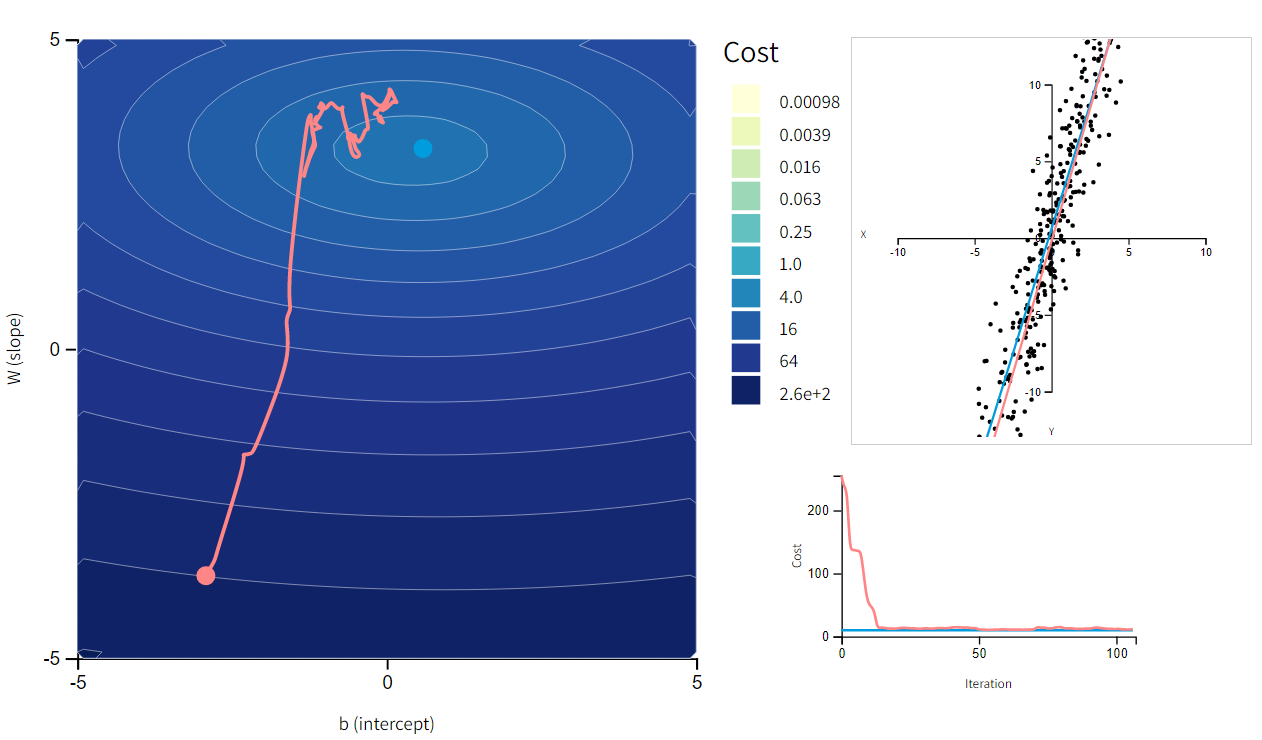
\includegraphics[width=7cm, height=4cm]{Figs/SGD.png}
		    \caption{Stochastic Gradient Descent, From Hands-on Machine Learning}
        \end{figure}
    \end{itemize}
\end{frame}

\begin{frame}{Gradient Descent Algorithm Types}
    \begin{itemize}
        \item Stochastic Gradient Descent
        \item Picks a random instance in the training set at every step
        \begin{figure}
            % \centering
            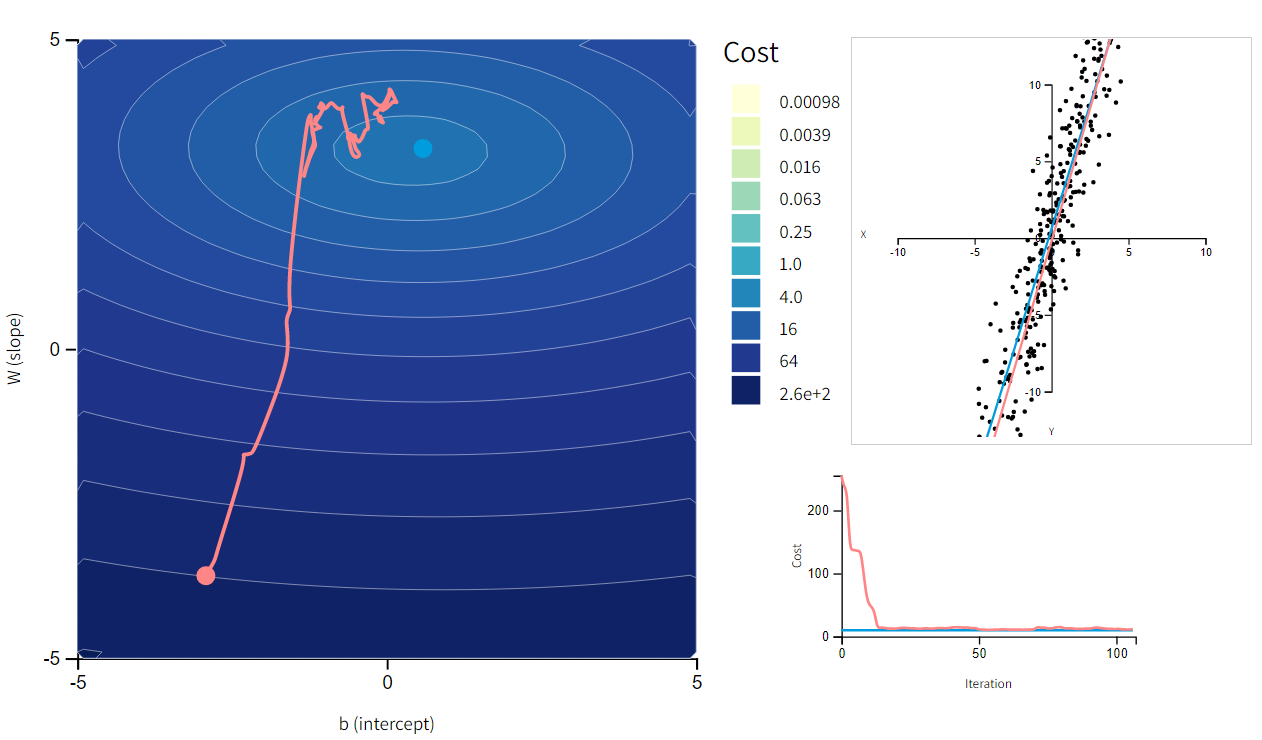
\includegraphics[width=7cm, height=4cm]{Figs/sgd.png}
		    \caption{Stochastic Gradient Descent Cost Function}
        \end{figure}
    \end{itemize}
\end{frame}